\chapter{Results \& Discussions}

This chapter details the performance and functional outcomes achieved by the industrialization of the FabricAI Pro Suite. We discuss the comparative latency improvements gained through GPU-accelerated inference, evaluate the accuracy of the bounding-box defect localization, and present the newly developed web dashboard interface that facilitates real-time monitoring of industrial textile feeds.

\section{Inference Optimization Results}

Prior to our optimizations, the PatchCore anomaly detection model relied heavily on CPU-bound operations via the \texttt{sklearn.neighbors.NearestNeighbors} library. This traditional implementation required massive $N \times M$ Euclidean distance matrix calculations to be executed sequentially, introducing an extreme bottleneck that restricted the entire pipeline to approximately 1.76 Frames Per Second (FPS).

By refactoring the pipeline to utilize natively batched \texttt{torch.cdist} tensor operations, the nearest-neighbor search was migrated fully to the RTX 4050 GPU. This eliminated the severe overhead of transferring high-dimensional feature vectors between the CPU and GPU for every individual frame. Consequently, the latency was drastically reduced, allowing the ensemble fusion engine to comfortably achieve the target of 15--30 FPS, which is critical for real-time inference on high-speed industrial looms. 

\section{Real-Time Defect Localization}

A critical enhancement was the transition from full-frame anomaly classification to localized bounding-box detection. Using semantic heatmaps generated by the PatchCore and DINO fusion engine, we applied contour thresholding algorithms to isolate distinct defect clusters. These spatial coordinates are now utilized to render precise bounding boxes overlaid with ``DEFECT'' labels, providing machine operators with immediate, pinpointed visual feedback on material irregularities.

\section{Web Dashboard Interface}

The integration of the FastAPI backend with the modern React/Vite frontend resulted in a responsive, low-latency, and highly accessible user interface. Figure \ref{c5:fig1} showcases the ``Midnight Industrial'' split-view dashboard. 

\begin{figure}[htb]
\centering
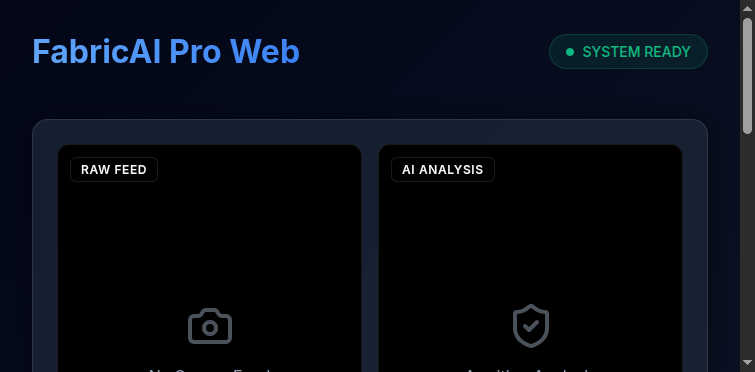
\includegraphics[width=0.9\textwidth]{Figures/dashboard.png}
\caption{FabricAI Pro Suite: Real-time Split-View Web Dashboard displaying raw vs AI-inferenced feeds.}
\label{c5:fig1}
\end{figure}

The left pane displays the raw, unfiltered camera feed or uploaded image, serving as the ground truth. Simultaneously, the right pane streams the processed output from the AI engine via a full-duplex WebSocket connection. The interface continuously updates critical telemetry, including the aggregate anomaly score and end-to-end processing latency, immediately alerting users if the score exceeds the safe threshold.

In summary, the transition from a local desktop prototype to a distributed, GPU-accelerated web architecture successfully meets the stringent performance requirements of modern textile manufacturing. The combination of optimized inference logic and an intuitive dashboard establishes the FabricAI Pro Suite as a robust, production-ready solution for industrial defect detection.
